\documentclass{article}
\usepackage{graphicx} % Required for inserting images
\usepackage{tikz}
\usetikzlibrary{positioning, backgrounds}
\usepackage{pfdicons}
\usepackage{mathtools}
\usepackage{empheq}
\usepackage{icomma}
\usepackage{siunitx}
\usepackage[a4paper, left=20mm, top=20mm]{geometry}
\usepackage[straightlabels, european, americanvoltages, cuteinductor]{circuitikz}
\usepackage{pgfplots}
\usepackage{subfig}
\usepackage{wrapfig}
\usepackage{float}
\usepackage{caption}
\usepackage{enumerate}
\usepackage{indentfirst}
\usepackage{marvosym}
\captionsetup{justification=raggedright,singlelinecheck=false}

\DeclareSIUnit{\voltac}{Vac}
\DeclareSIUnit{\voltdc}{Vdc}
\sisetup{output-decimal-marker = {,}}

\tikzset{background rectangle/.style={draw, dotted, line width=0.3mm}, background grid/.style={draw=gray, dotted, step=.5cm}}
\ctikzset{
fill=white, bipoles/cuteswitch/thickness=0.5
}

\renewcommand{\thefigure}{}
\renewcommand{\thesubfigure}{fig. \arabic{section}.\arabic{subsection}.\arabic{subfigure}}
\captionsetup[subfigure]{labelformat=simple,labelsep=colon,listofformat=subsimple}

\title{Electrónica General y Aplicada. Ejercicios de Práctica (TP1 a TP4)}
\author{Roberto Haarth, Tomás Vera. Facultad de Ingeniería, UNCuyo.}
\date{Septiembre 2025}

\begin{document}

\maketitle
\pagebreak

Se presentan ejercicios de resolución relacionados con los trabajos prácticos de la asignatura.

Estos ejercicios, algunos resueltos , cumplen con el objetivo de mejorar la capacidad y habilidad del estudiante en la comprensión y el logro 
de competencias en la asignatura de referencia

\begin{center}
    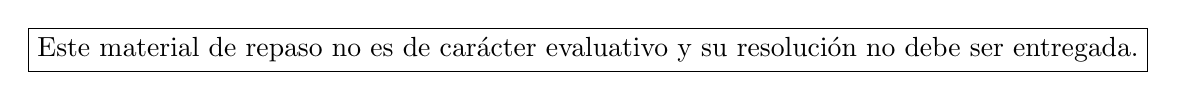
\begin{tikzpicture}
        \node[rectangle, draw, align=left]{Este material de repaso no es de carácter evaluativo y su resolución no debe ser entregada.};
    \end{tikzpicture}
\end{center}

\section{Trabajo Práctico 1: Reconocimiento de Componentes.}

\subsection{Divisor de tensión.}

El circuito posee una fuente $E_1$ y una resistencia $R_1$. La corriente que circula es $I_1 = \qty{50}{\milli\ampere}$. (\ref{fig:ej1a})

Luego se agrega una resistencia $R_2=\qty{100}{\ohm}$. $E_1$ permanece constante pero la corriente cambia a $I_2=\qty{40}{\milli\ampere}$. (\ref{fig:ej1b})


    \begin{wrapfigure}[2]{r}{0.6\textwidth}
        \vspace{-15mm}
        \centering
        \subfloat[]{
        \label{fig:ej1a}
            \begin{circuitikz}[show background rectangle, show background grid]
                \draw (0,0) to[vsource, invert, l=$E_1$] (0,3) -- (2,3)
                to[R, l_=$R_1$, i_>=$I_1$] (2,0) -- (0,0);
            \end{circuitikz}
        }
        \hspace{1mm}
        \subfloat[]{
        \label{fig:ej1b}
            \begin{circuitikz}[show background rectangle, show background grid]
                \draw (0,0) to[vsource, invert, l=$E_1$] (0,5) -- (2,5)
                to[R, l_=$R_1$, i>_=$I_2$] ++(0,-2.5) to[R, l_=$R_2$, a^=$\qty{100}{\ohm}$, i_>=$I_2$, *-] (2,0) -- (0,0);
                \draw[->] (2,2.5) -- ++(1,0) node[label=$V_S$]{};
            \end{circuitikz}
        }
    \end{wrapfigure}

\vspace{10mm}
\noindent\textbf{Determinar}:
\begin{enumerate}[A.]
    \item El valor de $V_S$ del divisor de tensión. (\ref{fig:ej1b})
    \item El valor de la fuente $E_1$.
    \item El valor de $R_1$.
\end{enumerate}
\vspace{15mm}

\setcounter{subfigure}{0}
\subsection{Divisor de tensión.}
Simplificar el circuito divisor de tensión. Indicar los valores de $V_{S1}$ y $V_{S2}$.
    \begin{figure}[H]
        \centering
        \subfloat[]{
        \label{fig:ej2}
            \begin{circuitikz}[show background rectangle, show background grid]
                \draw (0,-2) -- (0,0) to[vsource, invert, l=$\qty{12}{\volt}$] (0,4) -- (2,4)
                to[R, l=$R_1$] (2,2) -- (7,2)node[label=east:$V_{S1}$]{} to[open, *-*](7,-2)node[label=east:$\qty{0}{\volt}$]{} -- (0,-2);
                \draw (5,2) to[R, l=$R_3$, *-*] (5,0);
                \draw (2,2) to[vR, invert, l=$R_2$, *-*] (2,0) to[R, l=$R_4$, -*] (2,-2);
                \draw (4,0) to[R, l=$R_5$, *-*] (4,-2);
                \draw (6,0) to[R, l=$R_6$, *-*] (6,-2);
                \draw (0,0) to[short, *-*] (7,0)node[label=east:$V_{S2}$]{};
            \end{circuitikz}
        }
    \end{figure}
    \begin{center}
        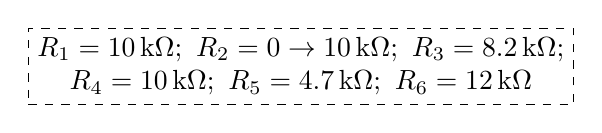
\begin{tikzpicture}
            \node[rectangle, draw, dashed, align=center]{$R_1=\qty{10}{\kilo\ohm};\ R_2=0\to\qty{10}{\kilo\ohm};\ R_3=\qty{8,2}{\kilo\ohm};$\\
            $R_4=\qty{10}{\kilo\ohm};\ R_5=\qty{4,7}{\kilo\ohm};\ R_6=\qty{12}{\kilo\ohm}$};
        \end{tikzpicture}
    \end{center}
    
\setcounter{subfigure}{0}
\subsection{Divisor de tensión.}
Calcule el valor de las resistencias para obtener $V_{S1}= 0 \to \qty{10}{\volt}$ y $V_{S2}=0 \to \qty{2,5}{\volt}$.

    \begin{figure}[H]
        \centering
        \subfloat[]{
        \label{fig:ej3}
            \begin{circuitikz}[show background rectangle, show background grid]
                \draw (0,-2) -- (0,0) to[vsource, invert, l=$\qty{10}{\volt}$] (0,4) -- (2,4)
                to[R, l=$R_1$] (2,2) -- (7,2)node[label=east:$V_{S1}$]{} to[open, *-*](7,-2)node[label=east:$0$V]{} -- (0,-2);
                \draw (5,2) to[R, l=$R_3$, *-*] (5,0);
                \draw (2,2) to[R, l=$R_2$, *-] (2,0) to[short, -*] (2,-2);
                \draw (4,0) to[R, l=$R_4$, -*] (4,-2);
                \draw (6,0) to[R, l=$R_5$, *-*] (6,-2);
                \draw (4,0) to[short, -*] (7,0)node[label=east:$V_{S2}$]{};
            \end{circuitikz}
        }
    \end{figure}

\setcounter{subfigure}{0}
\subsection{Divisor de tensión.}
Calcular la corriente $I_1$.

    \begin{figure}[H]
        \centering
        \subfloat[]{
        \label{fig:ej4}
            \begin{circuitikz}[show background rectangle, show background grid]
                \draw (0,0) to[vsource, invert, l=$\qty{14,4}{\volt}$, i_>=$I_1$] (0,3) -- (6,3)
                to[R, l=$R_5$] (6,0) -- (5,0) to[R, l_=$R_4$] (2,0) -- (0,0);
                \draw (1,3) -- (1,1.5) to[R, l=$R_6$] (1,0);
                \draw (2,3) to[R, l=$R_1$] (2,1.5) -- (2,0);
                \draw (5,3) to[R, l=$R_2$] (5,1.5) -- (5,0);
                \draw (2,1.5) to[R, l=$R_3$] (5,1.5);
            \end{circuitikz}
        }
    \end{figure}
    \begin{center}
        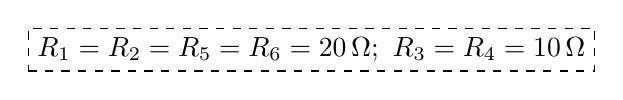
\begin{tikzpicture}
            \node[rectangle, draw, dashed, align=center]{$R_1=R_2=R_5=R_6=\qty{20}{\ohm};\ R_3=R_4=\qty{10}{\ohm}$};
        \end{tikzpicture}
    \end{center}

\setcounter{subfigure}{0}
\subsection{Divisor de tensión.}
Determinar la corriente $I_1$ y la tensión $V_{cb}$.

    \begin{figure}[H]
        \centering
        \subfloat[]{
        \label{fig:ej5}
            \begin{circuitikz}[show background rectangle, show background grid]
                \draw (0,0) to[vsource, invert, l=$\qty{12}{\volt}$] (0,3) to[short, i_>=$I_1$, -*] (3,3)
                to[R, l=$R_3$] (3,-1) -- (0,-1) -- (0,0);
                \draw (3,3) to[R, l_=$R_1$] ++(240:4.05) to[R, l=$R_2$] (3,-0.5);
                \draw (3,3) to[R, l=$R_4$] ++(-60:4.05) to[short, -*] (3,-0.5);
                \node at (1,-0.5)[circ, label=south west:c]{};
                \node at (3,-0.5)[circ, label=south east:b]{};
            \end{circuitikz}
        }
    \end{figure}
    \begin{center}
        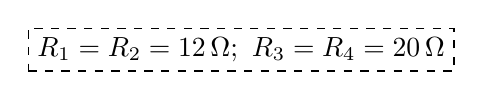
\begin{tikzpicture}
            \node[rectangle, draw, dashed, align=center]{$R_1=R_2=\qty{12}{\ohm};\ R_3=R_4=\qty{20}{\ohm}$};
        \end{tikzpicture}
    \end{center}

\pagebreak

\section{Trabajo Práctico 2: Rectificación y Filtrado.}
\setcounter{subfigure}{0}
\subsection{Circuito rectificador de media onda.}
\begin{enumerate}[A.]
    \item Graficar la señal en $a$ y $b$ cuando $S_1=\text{OFF}$ y $S_2=\text{OFF}$.
    \item Graficar la señal en $b$ cuando $S_1=\text{ON}$ y $S_2=\text{OFF}$.
    \item Graficar la señal en $c$ cuando $S_1=\text{ON}$ y $S_2=\text{ON}$.
    \item Graficar la señal en $c$ cuando $S_1=\text{OFF}$ y $S_2=\text{ON}$.
\end{enumerate}

    \begin{figure}[H]
        \centering
        \subfloat[]{
        \label{fig:ej6}
            \begin{circuitikz}[show background rectangle, show background grid]
                \draw node[transformer core, label=north:$T_1$](T){};
                \node at (T.west)[align=center]{\small220\\\small Vac};
                \node at (T.east)[align=center]{\small12\\\small Vac};
                \draw (T.B1) to[short,-*] ++(1,0)node[label=north:$a$](a){} to[D*] ++(1.5,0)node[label=north:$b$](b){};
                \draw (a.center) -- ++(0,-1.5) to[D*] ++(1.5,0);
                \draw (b.center) to[nos, l=$S_1$, *-] ++(0,-1.5);
                \draw (T.B2) to[short, -*] ++(1,0)node[ground]{} -- ++(3,0)node[](caplow){};
                \draw (b.center) -- ++(1.5,0)node[](capup){} to[nos, l=$S_2$, *-] ++(0,-1) to[ecapacitor, l2=$C_1$ and $\qty{470}{\micro\farad}$, -*] (caplow.center);
                \draw (capup.center) -- ++(2,0)node[label=north:$c$](c){} to[R, l2=$R_1$ and $\qty{1}{\kilo\ohm}$, *-] ++(0,-2) |- (caplow.center);
                
            \end{circuitikz}
        }
    \end{figure}

\setcounter{subfigure}{0}
\subsection{Circuito de rectificación de media onda y filtrado.}
La Experiencia de laboratorio da los resultados:
    \begin{center}
        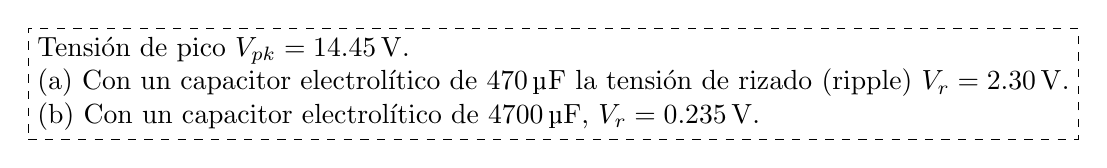
\begin{tikzpicture}
            \node[rectangle, draw, dashed, align=left]{Tensión de pico $V_{pk}=\qty{14,45}{\volt}$.\\
            (a) Con un capacitor electrolítico de \qty{470}{\micro\farad} la tensión de rizado (ripple) $V_r=\qty{2,30}{\volt}$.\\
            (b) Con un capacitor electrolítico de \qty{4700}{\micro\farad}, $V_r=\qty{0,235}{\volt}$.};
        \end{tikzpicture}
    \end{center}

Determinar:
\begin{enumerate}[A.]
    \item La tensión máxima y mínima para las dos situaciones (a y b).
    \item La tensión media para las dos situaciones.
    \item Qué condición debe cumplirse para que la tensión continua sea igual a la tensión de pico del rectificador. Fundamente.
\end{enumerate}

    \begin{figure}[H]
        \centering
        \subfloat[]{
        \label{fig:ej7}
            \begin{tikzpicture}[show background rectangle, show background grid]
                \begin{axis}[
                    ticks=none,
                    axis x line=middle,
                    axis y line=middle,
                    xscale=1.87, yscale=0.63,
                    ymax=70, ymin=-50,
                    xmin=10, xmax=13.2,
                    no marks,
                ]
                \addplot [blue!60, dashed, domain=10:14, samples=50,]{49.8};
                \addplot [blue!60, dashed, domain=10:14, samples=50,]{23};
                \addplot [red, very thin, domain=10:12.99, samples=100,]{49.8*sin(x*pi*115-15)};
                \addplot [blue, very thick] table [x="TIME", y="D3(A)", col sep=comma] {ripple2.DAT};
                \end{axis}
                
                \node at (0,3)[blue!75, anchor=east, outer sep=0pt]{$V_{max}$};
                \node at (0,2.25)[blue!75, anchor=east, outer sep=0pt]{$V_{min}$};
                \node at (2.5,0.5)[red, anchor=east, outer sep=0pt]{\Large$V_{AC}$};
                \node at (8,3)[blue, anchor=north, outer sep=0pt]{\Large$V_{DC}$};
                \draw[->, red!50!black] (5,1.5)node[label=south:\Large$V_{pk}$, inner sep=0pt]{} -- (5,3);
                \draw[<->, blue!75] (12,2.2) -- (12,3)node[blue!75, anchor=north west, outer sep=3pt]{\Large$V_{r}$};
            \end{tikzpicture}
        }
    \end{figure}

\pagebreak

\section{Trabajo Práctico 3: Transistor y Recta de Carga.}
\setcounter{subfigure}{0}
\subsection{Recta de carga.}
Determinar la recta de carga (valor de la ordenada y valor de la absisa) según los datos:
\begin{enumerate} [A.]
    \item Tensión de alimentación $V_{CC}=\qty{12}{\voltdc}$. Resistencia de carga $R_L=\qty{100}{\ohm}$. Corriente de base del transistor $I_B=\qty{100}{\micro\ampere}$.  Exprese los cálculos analíticos. Realice el gráfico.
    \item Tensión de alimentación $V_{CC}=\qty{12}{\voltdc}$. Resistencia de carga $R_L=\qty{200}{\ohm}$. Corriente de base del transistor $I_B=\qty{200}{\micro\ampere}$.  Exprese los cálculos analíticos. Realice el gráfico.
\end{enumerate}

\setcounter{subfigure}{0}
\subsection{Transistor en corte y saturación.}
Resolver para las figuras \ref{fig:ej9a} y \ref{fig:ej9b}.
\begin{enumerate}[A.]
    \item Indique el estado de los LED cuando la llave está abierta o cerrada.
    \item Realice una modificación al circuito para que los 2 LED estén en el mismo estado cuando la llave esté abierta o cerrada.
\end{enumerate}

    \begin{figure}[H]
        \centering
        \subfloat[]{
        \label{fig:ej9a}
            \begin{circuitikz}[show background rectangle, show background grid]
                \node at (0,0)[ground, label=east:GND](gnd1){};
                \node at (3,2)[npn](tran){};
                \draw (0,2) to[short](0.4,2) to[R, l=$R_2$](tran.B);
                \draw (gnd1.center) to[R,-*, a=$\qty{10}{\kilo\ohm}$](0,2) to[short](0,3) to[nos](0,4) to[R, a=$\qty{10}{\kilo\ohm}$](0,6) to[short,-*](3,6) to[R, a=$\qty{470}{\ohm}$](3,4) to[leD*,-*](tran.C);
                \draw (tran.E) to[short,*-*]++(3,0);
                \draw (tran.E) to[short](3,0)node[ground, anchor=center, label=east:GND]{};
                \draw (tran.C) to[R, a=$\qty{220}{\ohm}$]++(3,0) to[leD*]++(0,-1.5);
                \draw (3,6) -- (3,6.5)node[vcc, anchor=center, label=north:VCC]{};
            \end{circuitikz}
        }
        \subfloat[]{
        \label{fig:ej9b}
            \begin{circuitikz}[show background rectangle, show background grid]
                \node at (0,0)[ground, label=east:GND](gnd1){};
                \node at (3,2)[npn](tran){};
                \draw (0,2) to[short](0.4,2) to[R, l=$R_2$](tran.B);
                \draw (gnd1.center) to[R,-*, a=$\qty{10}{\kilo\ohm}$](0,2) to[short](0,3) to[nos](0,4) to[R, a=$\qty{10}{\kilo\ohm}$](0,6) to[short,-*](3,6) to[R, a=$\qty{470}{\ohm}$](3,4) to[leD*,-*](tran.C);
                \draw (tran.E) to[short,*-*]++(3,0);
                \draw (tran.E) to[short](3,0)node[ground, anchor=center, label=east:GND]{};
                \draw (tran.C) to[R, a=$\qty{220}{\ohm}$]++(3,0) to[leD*,invert]++(0,-1.5);
                \draw (3,6) -- (3,6.5)node[vcc, anchor=center, label=north:VCC]{};
            \end{circuitikz}
        }
    \end{figure}
\setcounter{subfigure}{0}
\subsection{Transistor en corte y saturación.}

Dado el circuito de la figura (el transistor trabaja en conmutación), indique el estado del LED según la posición de las llaves L1 y L2.

    \begin{figure}[H]
        \centering
        \subfloat[]{
        \label{fig:ej10}
            \begin{circuitikz}[show background rectangle, show background grid]
                \node at (3,2)[npn](tran){};
                \draw (0,2) to[short](0.4,2) to[R, l=$R_2$, a=$\qty{2200}{\ohm}$](tran.B);
                \draw (0,0) to[R,-*, a=$\qty{10}{\kilo\ohm}$](0,2) to[short](0,3) to[nos, l=L1](0,4) to[R, a=$\qty{10}{\kilo\ohm}$](0,6) to[short,-*](3,6) to[nos, l=L2](3,5) to[R, a=$\qty{500}{\ohm}$, -*](tran.C);
                \draw (tran.E) to[short](3,0)node[ground, anchor=center, label=east:GND](gnd){};
                \draw (0,0) to[short,-*] (gnd.center);
                \draw (tran.C) to[R, a=$\qty{220}{\ohm}$]++(3,0) to[leD*](6,0) -- (gnd.center);
                \draw (3,6) -- (3,6.5)node[vcc, anchor=center, label=north:VCC]{};
            \end{circuitikz}
        }
    \end{figure}

\setcounter{subfigure}{0}
\subsection{Curva característica del transistor.}
Indique cuál de las opciones es el circuito utilizado en la práctica para la determinación de la curva característica del transistor.

    \begin{figure}[H]
        \centering
        \subfloat[]{
        \label{fig:ej11a}
            \begin{circuitikz}[show background rectangle, show background grid]
                \node at (6.5,7.5)[circle, draw, fill=white]{\Large A};
                \node at (0,1)[ground](gnd1){};
                \node at (5,1)[ground](gnd2){};
                \node at (5,7)[vcc, anchor=center, label=north:$V_{CC}$, label=south west:$\qty{10}{\volt}$](vcc){};
                \draw[->] (4.75,7) -- (5.25,7.5);
                \node at (5,3.5)[pnp, yscale=-1](tran){};
                \draw (vcc.center) to[R, a=$\qty{500}{\ohm}$]++(0,-1.5) to[qiprobe, l_=$I_{C}$,-*](tran.C);
                \draw (gnd1.center) to[pR, name=pot, mirror, wiper pos=0.3](0,6) -- (0,7)node[vcc, label=north:$V_{DD}$, label=south east:$\qty{10}{\volt}$]{};
                \node at (pot.wiper)[anchor=north west, label=south:$\qty{4700}{\ohm}$, outer sep=1pt]{};
                \draw (pot.wiper) -- ++(0,0.225) to[R, a^=$\qty{2200}{\ohm}$](3,3.5) to[qiprobe, l=$I_B$]++(0.75,0)--(tran.B);
                \draw (tran.E) to[short,*-] ++(1.5,0)node[](emisor){};
                \draw (tran.C) -- ++(1.5,0) to[qvprobe, l_=$V_{CE}$](emisor.center);
                \draw (tran.B) to[short,*-]++(0,-0.5) to[qvprobe, l_=$V_{BE}$]++(0,-1.5) -| (gnd2.center);
                \draw (tran.E) to[short,-*](5,1.5);
            \end{circuitikz}
        }
        \subfloat[]{
            \label{ej11b}
            \begin{circuitikz}[show background rectangle, show background grid]
                \node at (6.5,7.5)[circle, draw, fill=white]{\Large B};
                \node at (0,1)[ground](gnd1){};
                \node at (5,1)[ground](gnd2){};
                \node at (5,7)[vcc, anchor=center, label=north:$V_{DD}$, label=south west:$\qty{10}{\volt}$](vcc){};
                \node at (5,3.5)[npn](tran){};
                \draw (vcc.center) to[R, a=$\qty{500}{\ohm}$]++(0,-1.5) to[qiprobe, l_=$I_{C}$,-*](tran.C);
                \draw (gnd1.center) to[pR, name=pot, mirror, wiper pos=0.3](0,6) -- (0,7)node[vcc, label=north:$V_{DD}$, label=south east:$\qty{10}{\volt}$]{};
                \node at (pot.wiper)[anchor=north west, label=south:$\qty{4700}{\ohm}$, outer sep=1pt]{};
                \draw (pot.wiper) -- ++(0,0.225) to[R, a^=$\qty{2200}{\ohm}$](3,3.5) to[qiprobe, l=$I_B$]++(0.75,0)--(tran.B);
                \draw (tran.E) to[short,*-] ++(1.5,0)node[](emisor){};
                \draw (tran.C) -- ++(1.5,0) to[qvprobe, l_=$V_{CE}$](emisor.center);
                \draw (tran.B) to[short,*-]++(0,-0.5) to[qvprobe, l_=$V_{BE}$]++(0,-1.5) -| (gnd2.center);
                \draw (tran.E) to[short,-*](5,1.5);
            \end{circuitikz}
        }
    \end{figure}
    \begin{figure}[H]
        \centering
        \subfloat[]{
        \label{fig:ej11c}
            \begin{circuitikz}[show background rectangle, show background grid]
                \node at (6.5,7.5)[circle, draw, fill=white]{\Large C};
                \node at (0,1)[ground](gnd1){};
                \node at (5,1)[ground](gnd2){};
                \node at (5,7)[vcc, anchor=center, label=north:$V_{DD}$, label=south west:$\qty{10}{\volt}$](vcc){};
                \node at (5,3.5)[pnp, yscale=-1](tran){};
                \draw (vcc.center) to[R, a=$\qty{500}{\ohm}$]++(0,-1.5) to[qiprobe, l_=$I_{C}$,-*](tran.C);
                \draw (gnd1.center) to[pR, name=pot, mirror, wiper pos=0.3](0,6) -- (0,7)node[vcc, label=north:$V_{DD}$, label=south east:$\qty{10}{\volt}$]{};
                \node at (pot.wiper)[anchor=north west, label=south:$\qty{4700}{\ohm}$, outer sep=1pt]{};
                \draw (pot.wiper) -- ++(0,0.225) to[R, a^=$\qty{2200}{\ohm}$](3,3.5) to[qiprobe, l=$I_B$]++(0.75,0)--(tran.B);
                \draw (tran.E) to[short,*-] ++(1.5,0)node[](emisor){};
                \draw (tran.C) -- ++(1.5,0) to[qvprobe, l_=$V_{CE}$](emisor.center);
                \draw (tran.B) to[short,*-]++(0,-0.5) to[qvprobe, l_=$V_{BE}$]++(0,-1.5) -| (gnd2.center);
                \draw (tran.E) to[short,-*](5,1.5);
            \end{circuitikz}
        }
        \subfloat[]{
            \label{ej11d}
            \begin{circuitikz}[show background rectangle, show background grid]
                \node at (6.5,7.5)[circle, draw, fill=white]{\Large D};
                \node at (0,1)[ground](gnd1){};
                \node at (5,1)[ground](gnd2){};
                \node at (5,7)[vcc, anchor=center, label=north:$V_{CC}$, label=south west:$\qty{12}{\volt}$](vcc){};
                \draw[->] (4.75,7) -- (5.25,7.5);
                \node at (5,3.5)[pnp, yscale=-1](tran){};
                \draw (vcc.center) to[R, a=$\qty{500}{\ohm}$]++(0,-1.5) to[qiprobe, l_=$I_{C}$,-*](tran.C);
                \draw (gnd1.center) to[pR, name=pot, mirror, wiper pos=0.3](0,6) -- (0,7)node[vcc, label=north:$V_{DD}$, label=south east:$\qty{10}{\volt}$]{};
                \node at (pot.wiper)[anchor=north west, label=south:$\qty{4700}{\ohm}$, outer sep=1pt]{};
                \draw (pot.wiper) -- ++(0,0.225) to[R, a^=$\qty{2200}{\ohm}$](3,3.5) to[qiprobe, l=$I_B$]++(0.75,0)--(tran.B);
                \draw (tran.E) to[short,*-] ++(1.5,0)node[](emisor){};
                \draw (tran.C) -- ++(1.5,0) to[qvprobe, l_=$V_{CE}$](emisor.center);
                \draw (tran.B) to[short,*-]++(0,-0.5) to[qvprobe, l_=$V_{BE}$]++(0,-2) -| (gnd2.center);
                \draw (tran.E) to[R,-*, a^=$\qty{220}{\ohm}$](5,1);
            \end{circuitikz}
        }
    \end{figure}
    \begin{center}
        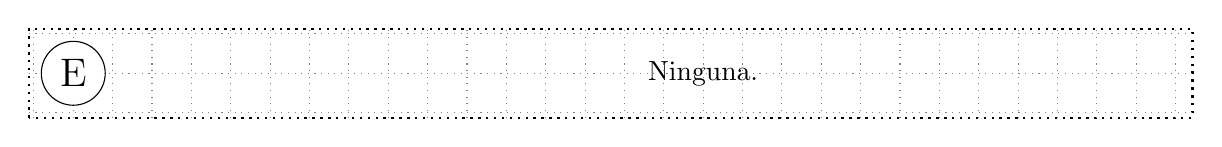
\begin{tikzpicture}[show background rectangle, show background grid]
            \node[rectangle, align=left, minimum width=\textwidth]{Ninguna.};
            \node at (-8,0)[circle, draw, fill=white]{\Large E};
        \end{tikzpicture}   
    \end{center}

\pagebreak
\section{Trabajo Práctico 4: Regulación de Tensión.}
\setcounter{subfigure}{0}
\subsection{Circuito regulador con diodo Zener.}
Calcular la Resistencia limitadora.

    \begin{figure}[H]
        \centering
        \subfloat[]{
        \label{fig:ej12}
            \begin{circuitikz}[show background rectangle, show background grid]
                \node at (0,0) [ground](gnd1){};
                \node at (2,0) [ground](gnd2){};
                \node at (4,0) [ground](gnd3){};
                \draw (gnd1.center) to[battery, invert, l2=$V_{CC}$ and $\qty{24}{\volt}$](0,3) to[R,-*, l=$R_{lim}$](2,3) -- (4,3) to[R, l=$R_C$](gnd3.center);
                \draw (gnd2.center) to[zzD*, l_=DZ1](2,3);
                \node at (5,3)[rectangle, draw, fill=white, dashed, anchor=north west, align=left]{
                $V_Z=\qty{12}{\volt}$\\
                $I_Z^{max}=\qty{76}{\milli\ampere}$\\
                $I_Z=0,5\,I_Z^{max}$\\
                $V_{CC}=\qty{24}{\volt}$\\
                $R_C=\qty{1200}{\ohm}$
               };
            \end{circuitikz}
        }
    \end{figure}

\setcounter{subfigure}{0}
\subsection{Circuito regulador con diodo Zener.}
Calcular la Tensión en el punto P cuando S1 está cerrada, casos A y B.

    \begin{figure}[H]
        \centering
        \subfloat[]{
        \label{fig:ej13}
            \begin{circuitikz}[show background rectangle, show background grid]
                \node at (0,-1) [ground](gnd1){};
                \draw (4,-1) to[R,*-, l=$R_2$](4,1) -- (6,1) to[R, l=$R_3$](6,-1);
                \draw (gnd1.center) to[battery, invert, l=$V_{CC}$](0,3) to[R,-*, l=$R_{lim}$](2,3) to[nos, l=S1](5,3) to[R, l=$R_1$](5,1)node[diamondpole, scale=1.5, label=south:\Large P]{};
                \draw (2,-1) to[zzD*, *-, l_=DZ1](2,3);
                \draw (6,-1) -- (0,-1);
            \end{circuitikz}
        }
    \end{figure}

    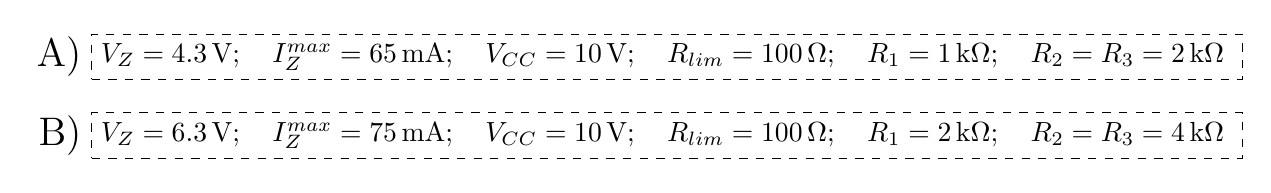
\begin{tikzpicture}
        \node[rectangle, draw, fill=white, dashed, anchor=north west, align=left, label=west:\Large A)](A){
                $V_Z=\qty{4,3}{\volt};\quad
                I_Z^{max}=\qty{65}{\milli\ampere};\quad
                V_{CC}=\qty{10}{\volt};\quad
                R_{lim}=\qty{100}{\ohm};\quad
                R_1=\qty{1}{\kilo\ohm};\quad
                R_2=R_3=\qty{2}{\kilo\ohm}$
               };
        \node[below=of A.west, rectangle, draw, fill=white, dashed, anchor=west, align=left, label=west:\Large B)](B){
                $V_Z=\qty{6,3}{\volt};\quad
                I_Z^{max}=\qty{75}{\milli\ampere};\quad
                V_{CC}=\qty{10}{\volt};\quad
                R_{lim}=\qty{100}{\ohm};\quad
                R_1=\qty{2}{\kilo\ohm};\quad
                R_2=R_3=\qty{4}{\kilo\ohm}$
               };
    \end{tikzpicture}

\setcounter{subfigure}{0}
\subsection{Circuito regulador con diodo Zener.}
Calcular $R_{lim}$ del circuito regulador con Zener. Considere que $V_Z$ regula.

    \begin{figure}[H]
        \centering
        \subfloat[]{
        \label{fig:ej14}
            \begin{circuitikz}[show background rectangle, show background grid]
                \node at (0,1) [ground](gnd1){};
                \node at (2,1) [ground](gnd2){};
                \node at (4,1) [ground](gnd3){};
                \draw (gnd1.center) to[battery, invert, l2=$V_{CC}$ and $\qty{18}{\volt}$](0,3) to[R,-*, l=$R_{lim}$](2,3) -- (4,3) to[R, l=$R_C$](gnd3.center);
                \draw (gnd2.center) to[zzD*, l_=DZ1](2,3);
                \node at (5,3)[rectangle, draw, fill=white, dashed, anchor=north west, align=left]{
                $V_{CC}=\qty{18}{\volt}$\\
                $V_Z=\qty{3,9}{\volt}$\\
                $I_Z^{max}=\qty{57,95}{\milli\ampere}$\\
                $I_Z^{min}=\qty{30}{\milli\ampere}$\\
                $R_Z=\qty{85}{\ohm}$\\
                $R_C=\qty{267}{\ohm}$
               };
            \end{circuitikz}
        }
    \end{figure}

\setcounter{subfigure}{0}
\subsection{Regulador de tensión ajustable.}
\begin{enumerate}
    \item Realice el circuito del regulador de tensión ajustable (ej. LM317). Indique las variables.
    \item Explique cómo se consigue ajustar la tensión de salida ($V_O$).
    \item ¿Cuál es el valor mínimo que se puede ajustar con el Regulador?
\end{enumerate}

\end{document}
